\documentclass[tikz,border=2pt]{standalone}
\usepackage{amsmath,amssymb}
\usepackage{tikz}
\usetikzlibrary{arrows.meta}

\begin{document}
% A power series centred at a converges absolutely inside (a-R, a+R), diverges outside, and the
% two endpoints must be checked one by one.
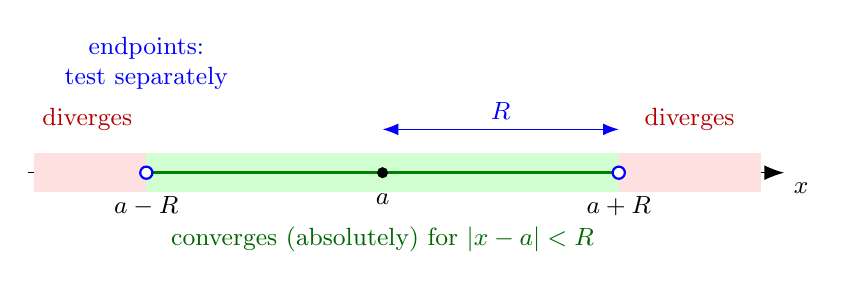
\begin{tikzpicture}[x=1.5cm, every node/.style={font=\small}]
	\draw[-{Latex[length=2.5mm]}] (-3,0) -- (3.4,0) node[below right] {$x$};
	\fill[green!18] (-2,-0.25) rectangle (2,0.25);
	\fill[red!12] (-2.95,-0.25) rectangle (-2,0.25);
	\fill[red!12] (2,-0.25) rectangle (3.2,0.25);
	\draw[very thick, green!50!black] (-2,0) -- (2,0);
	\fill[black] (0,0) circle (2pt) node[below=4pt] {$a$};
	\draw[blue, thick, fill=white] (-2,0) circle (2.2pt) node[below=5pt, black] {$a-R$};
	\draw[blue, thick, fill=white] (2,0) circle (2.2pt) node[below=5pt, black] {$a+R$};
	\draw[blue, {Latex[length=2mm]}-{Latex[length=2mm]}] (0,0.55) -- (2,0.55);
	\node[blue, above] at (1,0.55) {$R$};
	\node[green!40!black, below=16pt] at (0,0) {converges (absolutely) for $|x-a|<R$};
	\node[red!70!black, above=6pt] at (-2.5,0.2) {diverges};
	\node[red!70!black, above=6pt] at (2.6,0.2) {diverges};
	\node[blue, above=18pt, align=center] at (-2,0.3) {endpoints:\\ test separately};
\end{tikzpicture}
\end{document}
